\chapter{Implementacja}
\label{ch:implementacja}

Niniejszy rozdział przedstawia szczegóły implementacyjne systemu do przetwarzania i~archiwizacji strumieniowych danych
finansowych.
W~pierwszej części omówiono wykorzystane technologie wraz z~uzasadnieniem ich wyboru w~kontekście wymagań
zdefiniowanych w~rozdziale analizy.
Następnie przedstawiono napotkane problemy i~wyzwania, które wymagały zastosowania odpowiednich wzorców projektowych
i~optymalizacji.


\section{Wykorzystane technologie}
\label{sec:technologie}

Poniżej przedstawiono przegląd technologii wykorzystanych w~projekcie wraz z~uzasadnieniem ich wyboru.

\subsection{Język programowania Go}
\label{subsec:golang}

Go (Golang) został wybrany jako główny język implementacji ze względu na następujące cechy~\cite{go_at_google}:
\begin{itemize}
    \item Kompilacja do pojedynczego pliku wykonywalnego bez zewnętrznych zależności, co upraszcza dystrybucję
    i~budowanie obrazów Docker.
    \item Natywne wsparcie dla współbieżności poprzez gorutyny i~kanały, umożliwiające efektywną obsługę wielu
    połączeń WebSocket i~konsumentów wiadomości.
    \item Niski narzut pamięciowy i~szybki czas uruchamiania, istotne w~środowisku kontenerowym.
    \item Silne typowanie statyczne z~szybkim cyklem kompilacji.
    \item Bogate standardowe biblioteki sieciowe i~HTTP\@.
\end{itemize}

\subsection[Docker i Docker Compose]{Docker i~Docker Compose}
\label{subsec:tech_docker}

Konteneryzacja z~wykorzystaniem Docker zapewnia~\cite{docker}:
\begin{itemize}
    \item Izolację środowiska uruchomieniowego każdego komponentu.
    \item Powtarzalność budowy i~wdrożenia (obrazy są niemutowalne).
    \item Prostotę konfiguracji wielokomponentowego systemu poprzez Docker Compose.
    \item Łatwe skalowanie horyzontalne poprzez uruchamianie wielu instancji kontenera.
\end{itemize}

\begin{figure}[H]
    \centering
    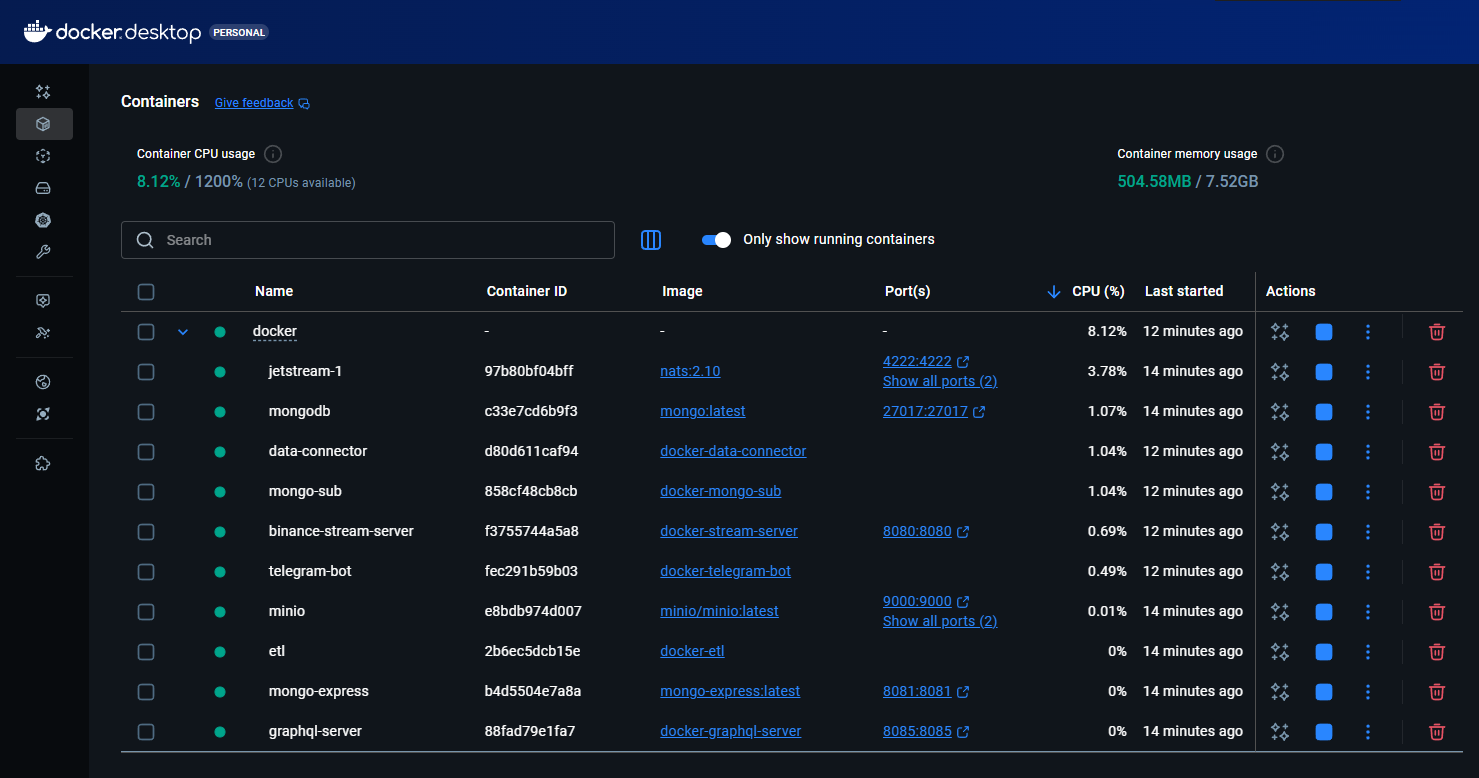
\includegraphics[width=0.85\textwidth,keepaspectratio]{rysunki/docker_desktop}
    \caption{Zestawienie aktywnych usług wchodzących w skład projektowanego systemu w środowisku Docker.}
    \label{fig:docker_desktop}
\end{figure}

\subsection{NATS JetStream}
\label{subsec:tech_nats}

NATS JetStream to rozproszony broker wiadomości zaprojektowany z~myślą o~wysokiej wydajności i~niskim opóźnieniu.
W~porównaniu do alternatyw takich jak Apache Kafka czy RabbitMQ, JetStream charakteryzuje się prostszą konfiguracją,
mniejszymi wymaganiami zasobowymi oraz natywnym wsparciem dla semantyki \textit{at-least-once} bez konieczności
zewnętrznej bazy danych~\cite{nats_jetstream_docs_persistence_at_least_once}.

NATS jest szczególnie odpowiedni dla scenariuszy wymagających niskich opóźnień, takich jak przetwarzanie danych
finansowych w~czasie rzeczywistym~\cite{time_value_curve}.

\subsection{MongoDB}
\label{subsec:tech_mongodb}

MongoDB to dokumentowa baza danych NoSQL, która zapewnia elastyczność schematu oraz wysoką wydajność zapisów~\cite{mongodb_manual}.
W~kontekście projektu, kluczowe zalety to:
\begin{itemize}
    \item Natywna obsługa dokumentów JSON, co eliminuje konieczność mapowania obiektowo-relacyjnego.
    \item Bogate możliwości agregacji danych (Aggregation Framework).
    \item Łatwa integracja z~językiem Go poprzez oficjalny sterownik.
\end{itemize}

W systemie MongoDB pełni rolę warstwy gorącej (\textit{hot storage}) przeznaczonej do szybkiego zapisu zdarzeń oraz
obsługi zapytań o~najnowsze dane.
Rysunki~\ref{fig:mongo_trade_record} oraz~\ref{fig:mongo_notification} przedstawiają strukturę kolekcji
oraz przykładowe rekordy.

\begin{figure}[H]
    \centering
    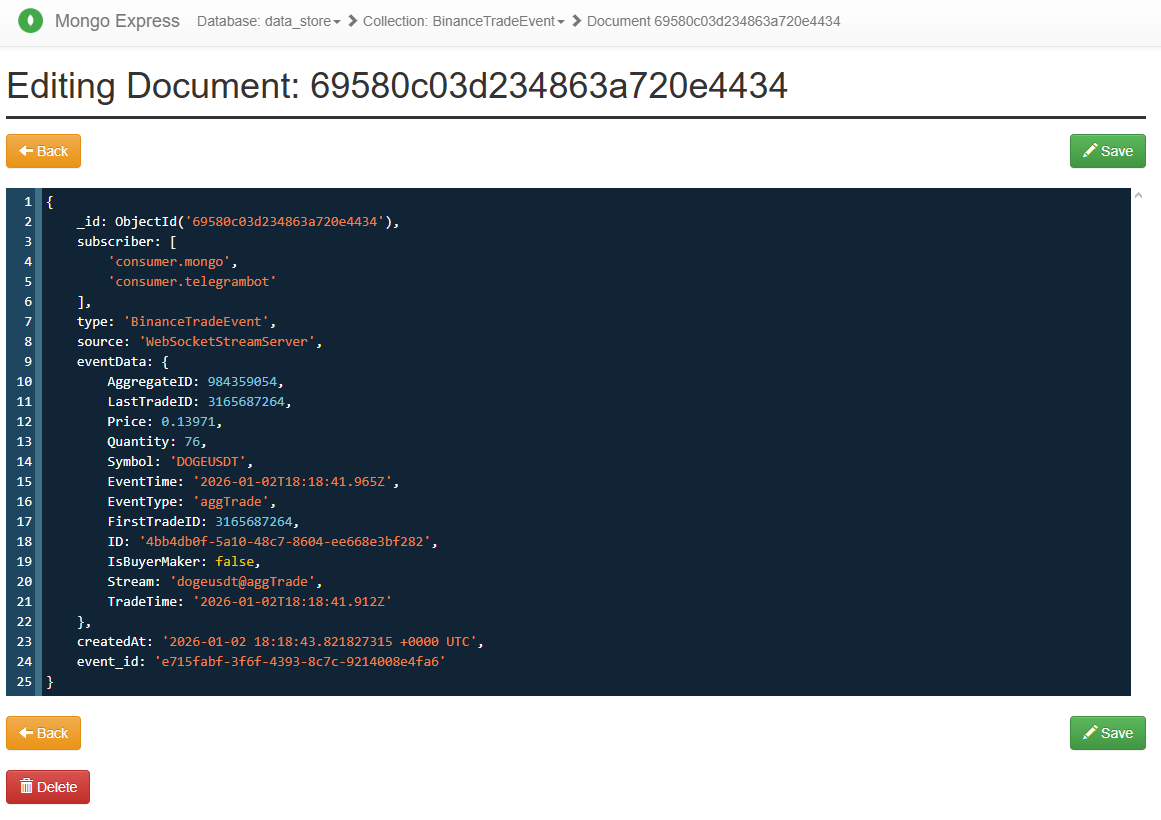
\includegraphics[width=0.85\textwidth,keepaspectratio]{rysunki/mongo_trade_record}
    \caption{Przykładowy rekord w~kolekcji BinanceTradeEvent zawierający pola domenowe transakcji oraz metadane.}
    \label{fig:mongo_trade_record}
\end{figure}

\begin{figure}[H]
    \centering
    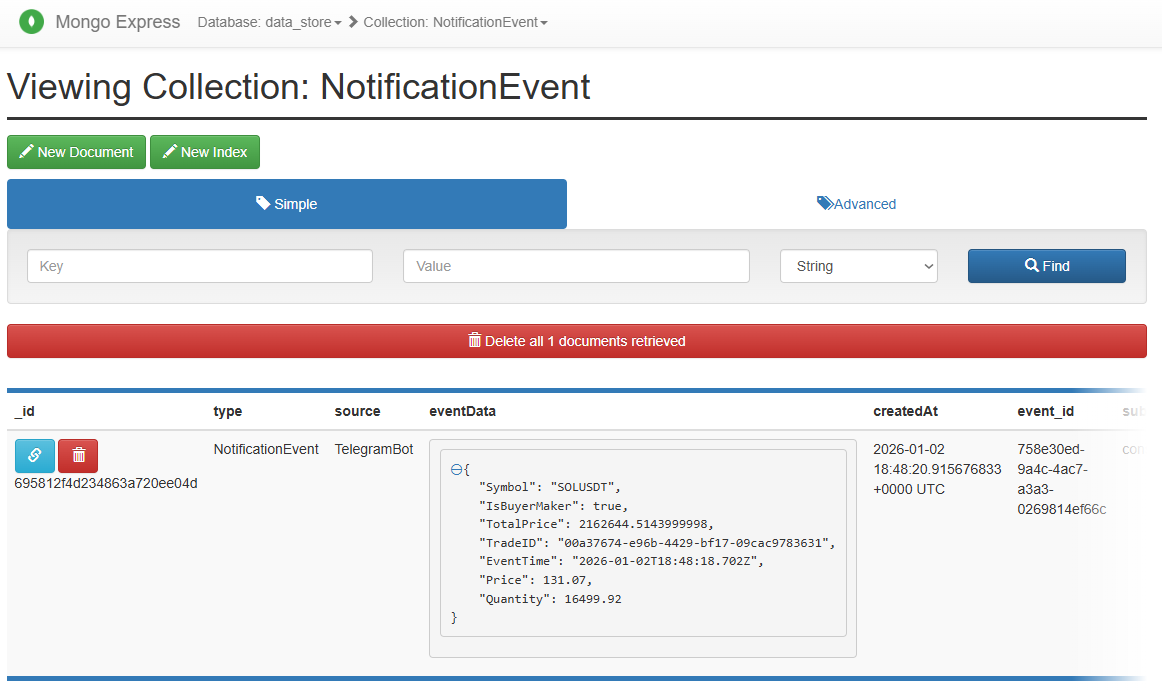
\includegraphics[width=0.85\textwidth,keepaspectratio]{rysunki/mongo_notification}
    \caption{Kolekcja NotificationEvent w~MongoDB przechowująca zdarzenia generowane przez system.}
    \label{fig:mongo_notification}
\end{figure}

\subsection{MinIO}
\label{subsec:tech_minio}

MinIO to wysokowydajny magazyn obiektowy kompatybilny z~protokołem Amazon S3.
Wybór MinIO podyktowany był możliwością uruchomienia w~środowisku lokalnym (\textit{on-premises}) bez zależności od
chmury publicznej, co jest kluczowe dla założeń projektu~\cite{cloud_repatriation_researchgate}.
MinIO zapewnia funkcje korporacyjne takie jak wersjonowanie, szyfrowanie i~replikacja, przy zachowaniu prostoty
wdrożenia w~kontenerze Docker~\cite{minio_docs}.

W ramach systemu MinIO pełni rolę warstwy zimnej (\textit{cold storage}) dla danych historycznych oraz warstwy
analitycznej.
Dane w~bucketach są organizowane w~sposób wspierający zarówno przetwarzanie przyrostowe, jak i~zapytania wsadowe.
Dla danych surowych zastosowano hierarchię katalogów według czasu (rok/miesiąc/dzień/godzina), natomiast dla danych
przetworzonych i~agregatów wykorzystano partycjonowanie w~stylu
klucz-wartość (np.\ symbol=DOGEUSDT/date=2025-12-05) w celu optymalizacji zapytań~\cite{hive_partitioning}.
Rysunki od~\ref{fig:minio_homepage} oraz~\ref{fig:minio_analytics_example} ilustrują zawartość bucketa binance-trades
w~MinIO oraz przykładową zawartość pliku z~agregatami czasowymi.

\begin{figure}[H]
    \centering
    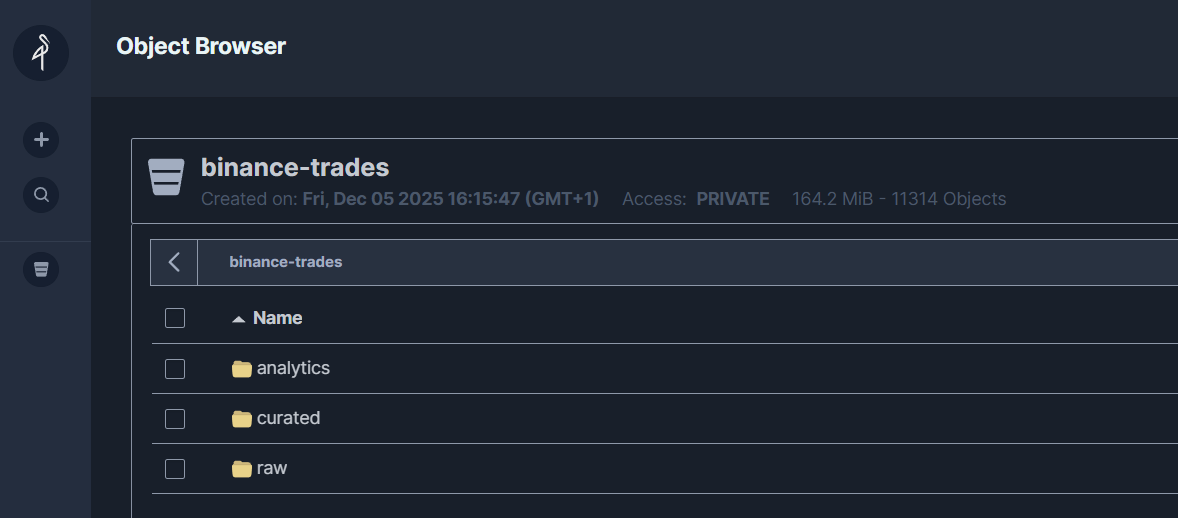
\includegraphics[width=0.85\textwidth,keepaspectratio]{rysunki/minio_homepage}
    \caption{Widok bucketa binance-trades w~MinIO z~podziałem na warstwy: raw (dane surowe), curated (dane
    oczyszczone) oraz analytics (agregaty).}
    \label{fig:minio_homepage}
\end{figure}

\begin{figure}[H]
    \centering
    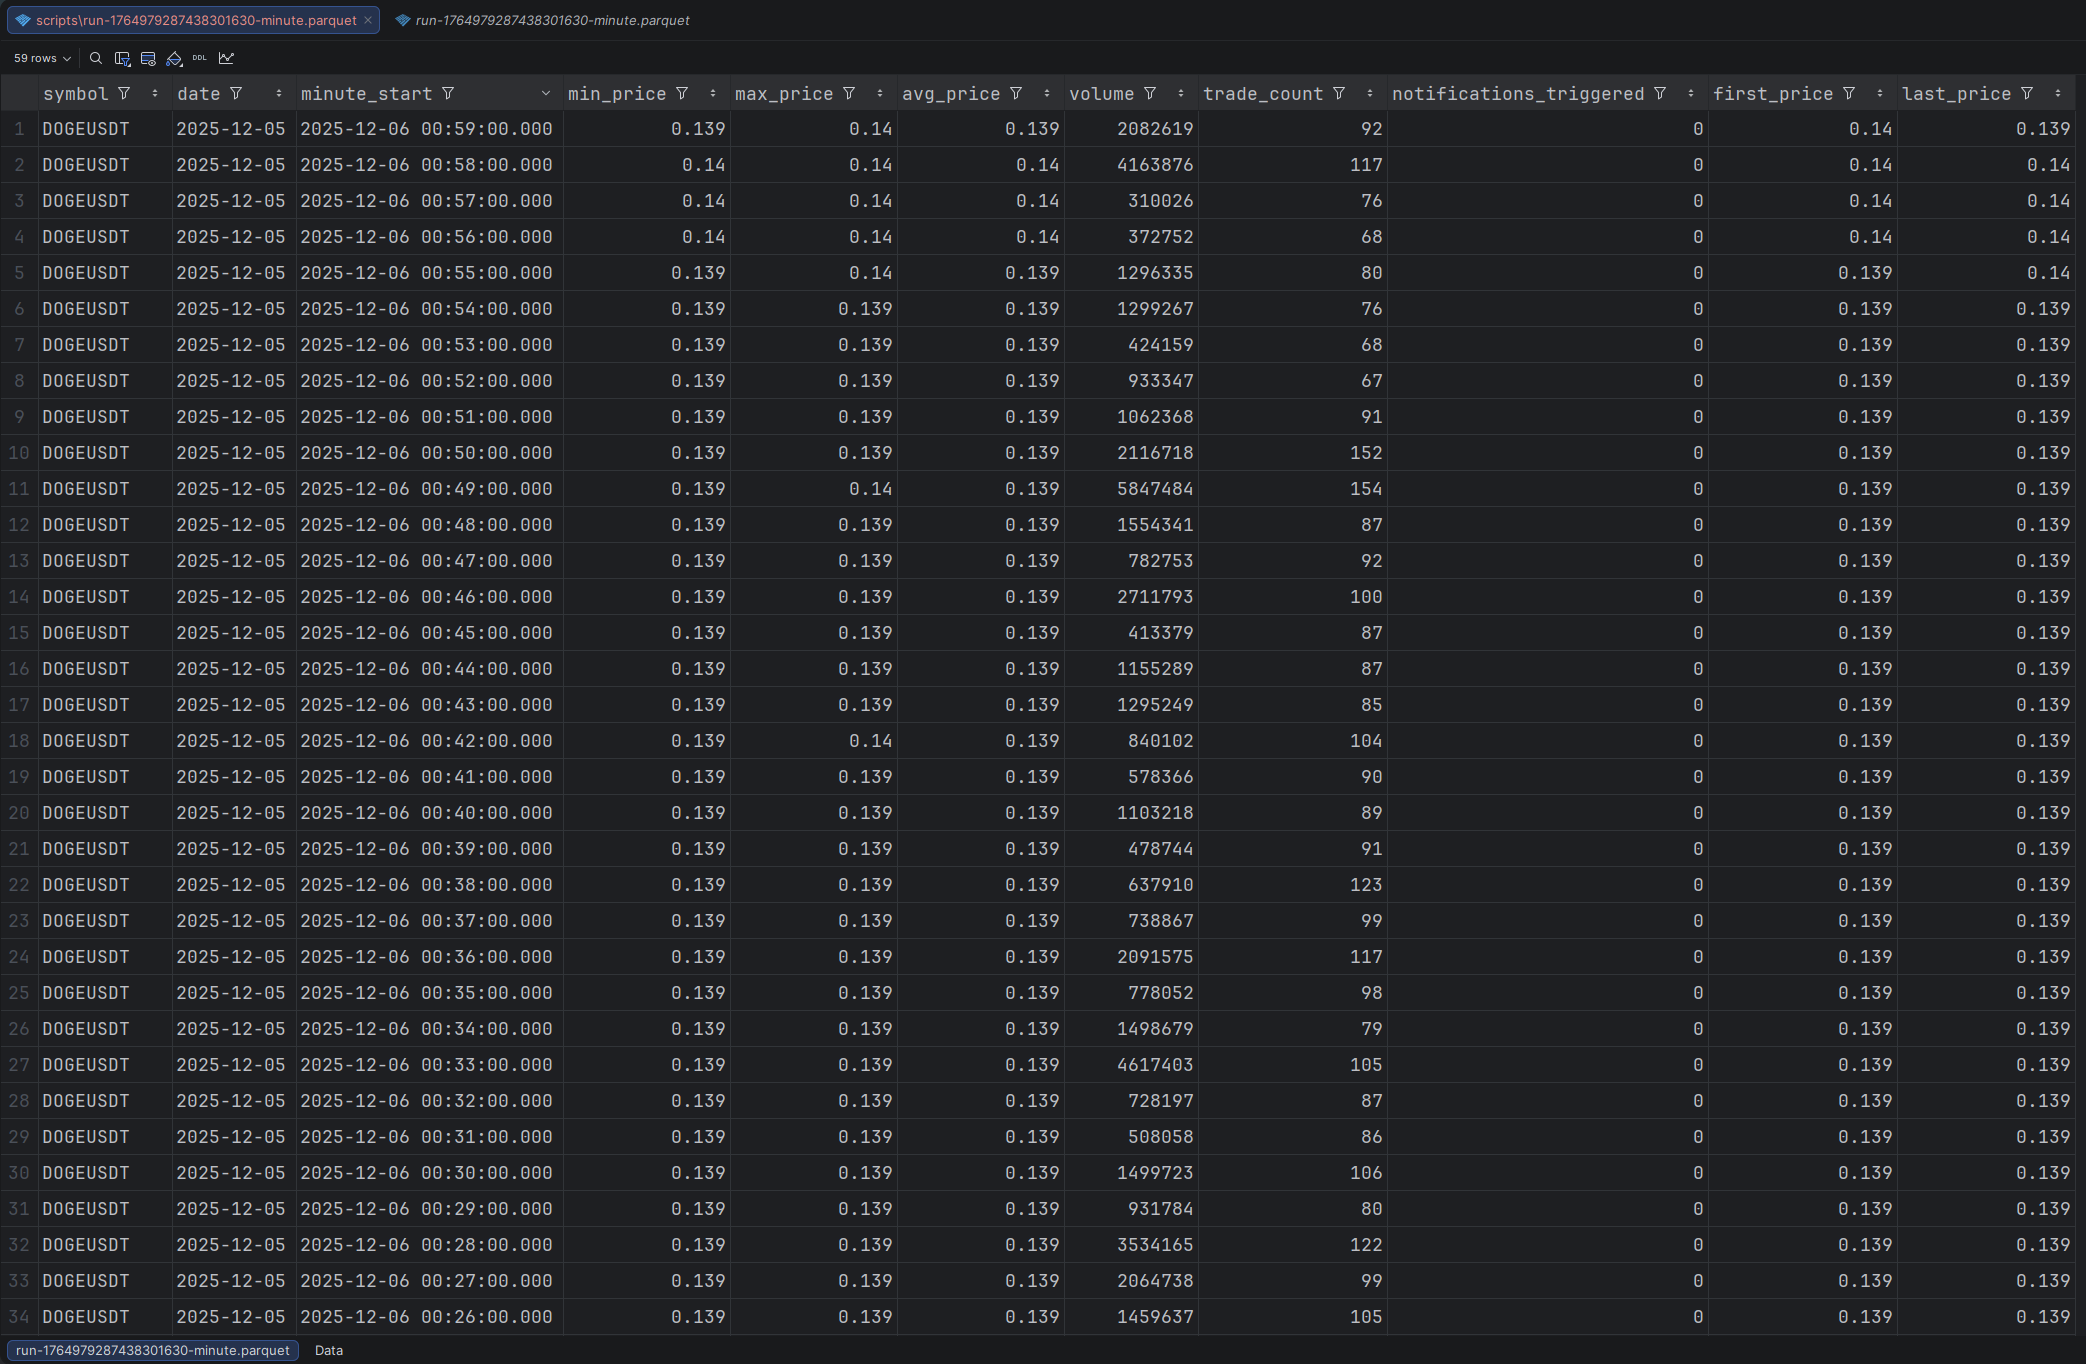
\includegraphics[width=0.85\textwidth,keepaspectratio]{rysunki/minio_analytics_example}
    \caption{Przykładowa zawartość pliku z~agregatami minutowymi w~warstwie analytics.}
    \label{fig:minio_analytics_example}
\end{figure}

\subsection[GraphQL i gqlgen]{GraphQL i~gqlgen}
\label{subsec:tech_graphql}

GraphQL to język zapytań do interfejsów API, który umożliwia klientom precyzyjne definiowanie struktury odpowiedzi.
Biblioteka gqlgen generuje typowany kod Go na podstawie schematu GraphQL, zapewniając spójność typów
w~czasie kompilacji oraz wysoką wydajność dzięki unikaniu refleksji w~czasie wykonania~\cite{graphql_docs}.

Schemat GraphQL zapisywany jest w~postaci SDL (\textit{Schema Definition Language}), czyli deklaratywnej definicji
obiektów domenowych, typów wejściowych (\textit{input}) oraz dostępnych operacji (\textit{query}).
W~SDL znak wykrzyknika oznacza pole wymagane (\textit{non-null}), tzn.\ serwer gwarantuje, że wartość nie
będzie pusta.
Z~kolei nawiasy kwadratowe oznaczają listę elementów~\cite{gqlgen_docs}.

Poniższy zrzut ekranu (Rysunek~\ref{fig:gql_query_example_0}) przedstawia przykładowe zapytanie GraphQL, które ilustruje
elastyczność API w~zakresie doboru pól oraz warunków filtrowania.

\begin{figure}[H]
    \centering
    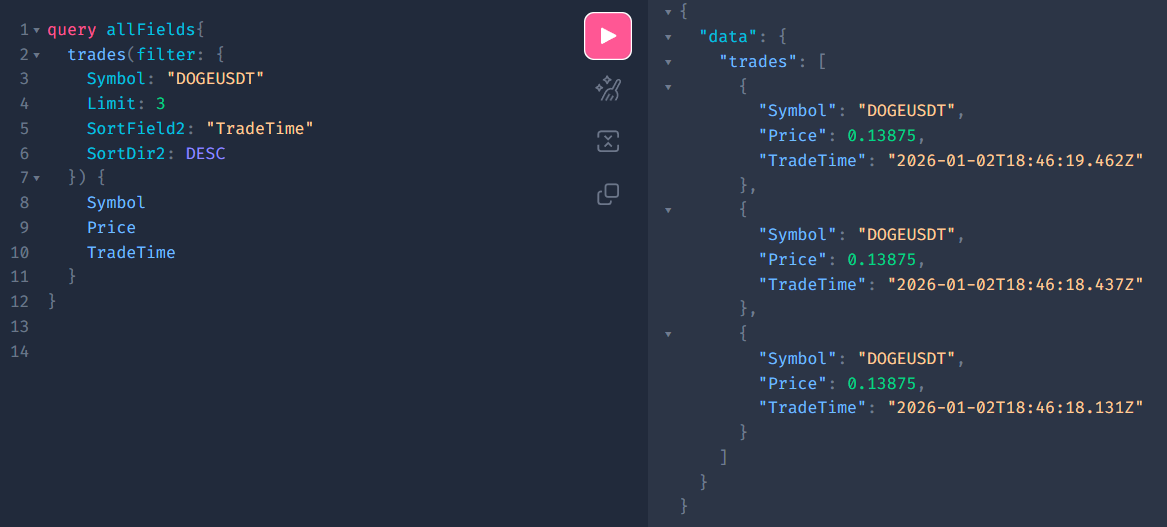
\includegraphics[width=0.85\textwidth,keepaspectratio]{rysunki/gql_query_example_0}
    \caption{Przykładowe zapytanie: trzy najnowsze zdarzenia dla symbolu DOGEUSDT\@.}
    \label{fig:gql_query_example_0}
\end{figure}

\subsection[Modele danych w języku Go]{Modele danych w~języku Go}
\label{subsec:tech_models}

Warstwa modeli w~języku Go opisuje struktury danych wykorzystywane na kolejnych etapach potoku: od~danych wejściowych
z~WebSocket, przez zdarzenia zapisywane w~bazie, aż po~dane przygotowane do archiwizacji w~magazynie obiektowym.
Jawne typy struktur stanowią kontrakt między mikroserwisami oraz ograniczają liczbę błędów integracyjnych dzięki
weryfikacji typów w~czasie kompilacji.
Rysunek~\ref{fig:model_data} przedstawia strukturę (\textit{BinanceTradeData}) wykorzystywaną do~reprezentacji danych
odebranych z~WebSocket.

\begin{figure}[H]
    \centering
    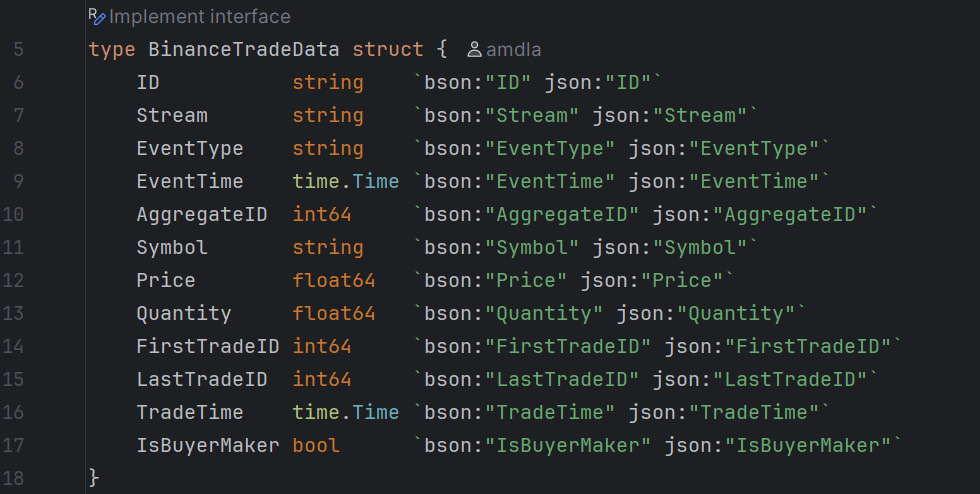
\includegraphics[width=0.65\textwidth,keepaspectratio]{rysunki/model_data}
    \caption{Struktura BinanceTradeData --- podstawowy model danych transakcyjnych pobierany z~WebSocket.}
    \label{fig:model_data}
\end{figure}

\subsection{Format Parquet}
\label{subsec:tech_parquet}

Apache Parquet to kolumnowy format przechowywania danych, zoptymalizowany pod kątem analitycznych obciążeń odczytu.
Kluczowe zalety~\cite{apache_parquet_docs}:
\begin{itemize}
    \item Efektywna kompresja kolumnowa (często 10x redukcja rozmiaru względem JSON).
    \item Szybkie odczyty selektywne (tylko wybrane kolumny są dekompresowane).
    \item Wsparcie dla złożonych schematów z~zagnieżdżonymi strukturami.
    \item Szeroka kompatybilność z~narzędziami analitycznymi (Pandas, Spark, DuckDB).
\end{itemize}

\subsection{Viper}
\label{subsec:tech_viper}

Viper to biblioteka Go do zarządzania konfiguracją, wspierająca wiele źródeł z~możliwością hierarchicznego
nadpisywania.
Umożliwia elastyczne konfigurowanie mikroserwisów bez konieczności rekompilacji~\cite{viper_lib}.

\subsection[Jupyter Notebook i Python]{Jupyter Notebook i~Python}
\label{subsec:tech_jupyter}

Jupyter Notebook służy jako interfejs do eksploracyjnej analizy danych historycznych przechowywanych w~MinIO\@.
Środowisko Python z~bibliotekami Pandas, PyArrow i~scikit-learn umożliwia~\cite{jupyter_docs}:
\begin{itemize}
    \item Interaktywną eksplorację zbiorów danych.
    \item Wizualizację trendów i~anomalii.
    \item Prototypowanie modeli uczenia maszynowego.
    \item Generowanie raportów analitycznych.
\end{itemize}


\section[Problemy i wyzwania]{Problemy i~wyzwania}
\label{sec:problemy_wyzwania}

Realizacja systemu o~architekturze rozproszonej wiąże się z~szeregiem wyzwań projektowych i~implementacyjnych,
które wymagają świadomych kompromisów oraz zastosowania odpowiednich wzorców i~praktyk inżynierskich.
Poniżej przedstawiono kluczowe problemy zidentyfikowane w~trakcie projektowania i~implementacji systemu.

\subsection{Złożoność architektury mikrousługowej}
\label{subsec:zlozonosc_mikrouslug}

Architektura mikrousługowa, pomimo licznych zalet takich jak niezależne skalowanie i~wdrażanie, wprowadza znaczącą
złożoność operacyjną.
Każdy mikroserwis wymaga własnej konfiguracji, zarządzania zależnościami, obsługi błędów oraz monitorowania.
Liczba potencjalnych punktów awarii rośnie proporcjonalnie do liczby komponentów, co wymaga wdrożenia strategii
odporności (\textit{resilience patterns}).

Komunikacja między serwisami poprzez sieć wprowadza dodatkowe źródła opóźnień i~błędów (timeouty, utrata połączenia,
przeciążenie), które muszą być obsługiwane na poziomie aplikacji.
W~tradycyjnych systemach monolitycznych, wywołania między modułami realizowane są w~ramach jednego procesu, co
eliminuje tę klasę problemów~\cite{newman_building_microservices}.

\subsection[Debugowanie i śledzenie rozproszone]{Debugowanie i~śledzenie rozproszone}
\label{subsec:debugowanie}

Diagnostyka problemów w~systemie rozproszonym jest znacząco bardziej złożona niż w~aplikacji monolitycznej.
Pojedyncze żądanie użytkownika może przepływać przez wiele usług, a~logi każdej z~nich muszą zostać skorelowane
w~celu odtworzenia pełnego obrazu sytuacji.
Wymaga to implementacji mechanizmów propagacji kontekstu (np.\ identyfikatorów korelacji) oraz centralizacji logów.

Dodatkowo, błędy związane z~kolejnością zdarzeń są trudniejsze do reprodukcji w~środowisku rozproszonym, gdzie czas
wykonania poszczególnych operacji zależy od wielu czynników zewnętrznych~\cite{open_telemetry}.

\subsection{Przetwarzanie sterowane zdarzeniami}
\label{subsec:event_driven_challenges}

Paradygmat \textit{Event-Driven Architecture} wymaga odmiennego podejścia do projektowania niż tradycyjne systemy
oparte na synchronicznych wywołaniach.
Należy precyzyjnie zdefiniować strukturę zdarzeń (kontrakty), zapewnić wersjonowanie schematów oraz obsłużyć
scenariusze takie jak zdarzenia niespójne czasowo (\textit{out-of-order events}) czy zduplikowane komunikaty~\cite{at_least_once}.

\subsection{Zarządzanie wieloma kontenerami}
\label{subsec:zarzadzanie_kontenerami}

System składa się z~wielu kontenerów Docker, których uruchomienie i~koordynacja wymaga odpowiedniej konfiguracji
orkiestracji.
Proces uruchamiania pełnego środowiska deweloperskiego jest czasochłonny (kilka minut), co wydłuża cykl
debugowania --- nawet drobna literówka w~kodzie wymaga przebudowania obrazu i~restartu kontenera.

Ponadto, duża liczba kontenerów i~wolumen przetwarzanych danych przekładają się na znaczące wymagania zasobowe.
Optymalizacja wykorzystania pamięci i~procesora jest niezbędna do uruchomienia systemu na typowej stacji roboczej
dewelopera.

\subsection[Jednoczesny dostęp do danych historycznych i bieżących]{Jednoczesny dostęp do danych historycznych i~bieżących}
\label{subsec:dostep_danych}

Specyficznym wyzwaniem jest zapewnienie jednoczesnego dostępu do danych w~dwóch warstwach o~odmiennych
charakterystykach.
Warstwa gorąca (MongoDB) optymalizowana jest pod kątem szybkich zapisów i~zapytań punktowych, natomiast warstwa
zimna (MinIO) przeznaczona jest do sekwencyjnego odczytu dużych zbiorów danych.

\subsection{Projektowanie elastycznego API}
\label{subsec:projektowanie_api}

Zaprojektowanie interfejsu GraphQL umożliwiającego elastyczne zapytania z~wieloma filtrami wymagało głębokiego
zrozumienia specyfiki tego standardu.
GraphQL różni się znacząco od REST pod względem modelowania danych, obsługi błędów oraz optymalizacji wydajności~\cite{graphql_docs}.

Dodatkowo, biblioteka gqlgen wymaga zdefiniowania schematu w~języku SDL (\textit{Schema Definition Language}),
a~następnie implementacji (\textit{resolverów}) --- funkcji odpowiedzialnych za pobieranie danych dla poszczególnych pól~\cite{gqlgen_docs}.

\subsection{Optymalizacja procesu archiwizacji}
\label{subsec:optymalizacja_archiwizacji}

Efektywne przenoszenie danych między warstwami wymaga starannej optymalizacji pod kątem wykorzystania zasobów
sieciowych i~dyskowych.
Proces musi być realizowany przyrostowo, bez blokowania bieżących operacji, z~mechanizmem wznawiania w~przypadku
przerwania.

Kompresja danych do formatu Parquet jest operacją kosztowną obliczeniowo, dlatego należy wyważyć stopień kompresji
(a~co za tym idzie oszczędność miejsca) z~czasem wykonania procesu archiwizacji.

